\documentclass[acmlarge]{acmart}


% customized
\usepackage[utf8]{inputenc}
\usepackage{xspace}
\usepackage{xcolor}
\usepackage{graphicx}

\usepackage{pifont}
\usepackage{amsmath}
\usepackage{amsfonts}
\let\Bbbk\relax         % avoid amssymb conflicting with other modern pkgs
\usepackage{amssymb}    % for \varnothing
\usepackage{algorithm}
\usepackage{algorithmicx}
\usepackage{algpseudocode}
\usepackage{enumitem}
\usepackage{tikz}
\usepackage{url}
\usepackage{lipsum} % for dummy text only

\usepackage{graphicx}
\graphicspath{{images/}{figures/}}

%%% choose from either subfigure, or caption + subcaption
%\usepackage{subfigure}
%% \begin{figure}
%%   \subfigure[caption]{
%       \include ...
%       \label
%    }
%% \end{figure}
\usepackage{caption}
\usepackage{subcaption}
%% \begin{figure}
%%   \begin{subfigure}[]{.8\columnwidth}
%%   \include ...
%%   \label ...
%%   \caption{...}
%%   \end{subfigure}
%% \end{figure}

% NEW coding style
%% need python pygments package: brew install pygments
\usepackage{minted}
\usemintedstyle{manni}
\renewcommand\theFancyVerbLine{\footnotesize\arabic{FancyVerbLine}}
\setminted{
    mathescape,
    frame=none,
    framesep=2mm,
    fontsize=\footnotesize,
    linenos,
    numbersep=5pt,
    numbers=left,
    tabsize=2,
    autogobble,
    xleftmargin=0.4cm,
}

% OLD coding style
\usepackage{listings}
\usepackage{color}
\lstset{
  basicstyle=\footnotesize\ttfamily,
  frame=none,	% none, single
  numbers=left,
  language=C,
  xleftmargin=0.4cm,
  showstringspaces=false,
  numbersep=5pt,
  numberstyle=\footnotesize\color{black},
  tabsize=2
}
% xleftmargin=0.25in

\newcommand{\paragraphb}[1]{\vspace{1mm}\noindent{\bf #1.}\quad}

%% tikz: circled texts
\newcommand*\circled[1]{\tikz[baseline=(char.base)]{\node[shape=circle,draw,inner sep=1pt] (char) {\scriptsize #1};}}

%% custom editing commands
\newcommand{\todo}[1]{\textcolor{red}{[TODO: #1]}}

%% system name
\def\sys{SysName\xspace}

%% chinese support:
%%%% 1. only work with xeLaTeX (instead of pdfLaTeX)
%%%% 2. does not work with the USENIX template
%%%% 3. simply type UTF-8 traditional chinese characters in the document
%%%% 4. to build, use 'latexmk -pdfxe'
\iffalse	% iffalse or iftrue
\usepackage[BoldFont, SlantFont, CJKchecksingle, CJKmath=true]{xeCJK}
\setCJKmainfont{AR PL KaitiM Big5}
\setCJKsansfont{AR PL Mingti2L Big5}
\XeTeXlinebreaklocale "zh"
\XeTeXlinebreakskip = 0pt plus 1pt
\fi



\AtBeginDocument{%
  \providecommand\BibTeX{{%
    \normalfont B\kern-0.5em{\scshape i\kern-0.25em b}\kern-0.8em\TeX}}}

\setcopyright{acmcopyright}
\copyrightyear{2023}
\acmYear{2023}
\acmDOI{10.1145/3437881}    % to be filled

\acmJournal{TOMM}
\acmVolume{17}
\acmNumber{2}
\acmArticle{54}
\acmMonth{6}

\begin{document}

\title{\sys: Paper Title}

\iffalse
\author{Anonymous Authors}
\authornotemark[1]
\email{anonymous@institution.com}
\affiliation{%
  \institution{Anonymous Institution}
  \city{Anonymous City}
  \country{Anonymous Country}
%  \postcode{43017-6221}
}
\fi

%\iffalse
\author{Your Name}
\authornotemark[1]
\email{email@nycu.edu.tw}
\affiliation{%
  \institution{National Yang Ming Chiao Tung University}
  \city{Hsinchu}
  \country{Taiwan}
%  \postcode{30010}
}

\author{Chun-Ying Huang}
\authornotemark[1]
\email{chuang@cs.nycu.edu.tw}
\affiliation{%
  \institution{National Yang Ming Chiao Tung University}
  \city{Hsinchu}
  \country{Taiwan}
%  \postcode{30010}
}
%\fi

\begin{CCSXML}
<ccs2012>
<concept>
<concept_id>10002978.10002997.10002998</concept_id>
<concept_desc>Security and privacy~Malware and its mitigation</concept_desc>
<concept_significance>500</concept_significance>
</concept>
<concept>
<concept_id>10002978.10002997.10002999</concept_id>
<concept_desc>Security and privacy~Intrusion detection systems</concept_desc>
<concept_significance>300</concept_significance>
</concept>
<concept>
<concept_id>10002978.10003006.10011634</concept_id>
<concept_desc>Security and privacy~Vulnerability management</concept_desc>
<concept_significance>500</concept_significance>
</concept>
<concept>
<concept_id>10002978.10003022</concept_id>
<concept_desc>Security and privacy~Software and application security</concept_desc>
<concept_significance>500</concept_significance>
</concept>
</ccs2012>
\end{CCSXML}

\ccsdesc[500]{Security and privacy~Malware and its mitigation}
\ccsdesc[300]{Security and privacy~Intrusion detection systems}
\ccsdesc[500]{Security and privacy~Vulnerability management}
\ccsdesc[500]{Security and privacy~Software and application security}

\begin{abstract}
TBW---Write your abstracts here.

\end{abstract}

\keywords{Keyword1, Keyword2, Keyword3}

\maketitle


\section{Introduction}
\label{sec:intro}

Write introduction here ... reference to Figure~\ref{fig:symbols}, and cite a paper~\cite{HCHFC21}.

\begin{figure}
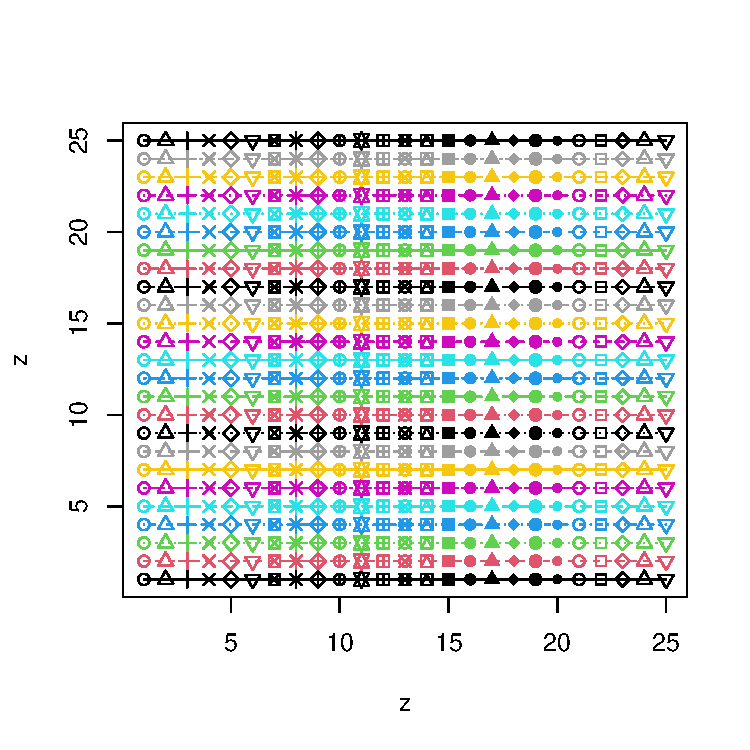
\includegraphics[width=.99\columnwidth]{images/symbols.pdf}
\caption{Symbols.}
\label{fig:symbols}
\end{figure}


\section{Related Work}
\label{sec:related}

Write related works here.


\section{Background}
\label{sec:back}

\subsection{Sub-Section 1}
\label{subsec:back_one}

Write paper background or objectives here.


\section{Approach}
\label{sec:approach}

Write your approach here.

\begin{figure}
\begin{minted}[breaklines]{c}
#include <stdio.h>

int main() {
    printf("hello, world!\n");
    return 0;
}
\end{minted}
\caption{Sample {\tt hello, world!} program.}
\label{fig:hello_world}
\end{figure}

\section{Evaluation}
\label{sec:eval}

Write evaluation here.


\section{Conclusion}
\label{sec:conclusion}

Write conclusion here.





\bibliographystyle{ACM-Reference-Format}
\bibliography{main}

\end{document}
